\chapter{Model der Bildaufnahme mit einer Kamera }
\label{sec:CameraModels}

Um einen Szenenrekonstruktionalgorithmus zu verstehen werden in diesem Abschnitt grundlegende  Bedingungen eingeführt um die Bildaufnahme mathematisch zu beschreiben. Ein abbildendes System besteht aus einem Objekt $M$, einer Kamera $C$ und einer Bildebene $I$ wie in Abbildung \ref{fig:PinholeCamera3D} dargestellt.\\



\begin{figure}[!htb]
	\centering
	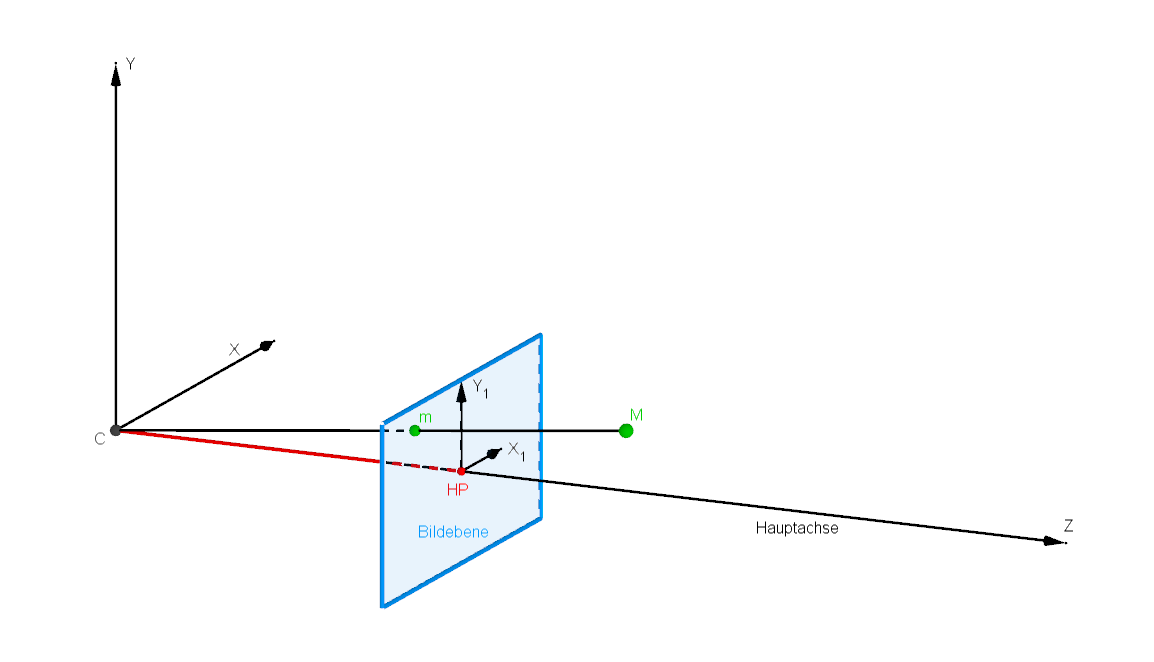
\includegraphics[width=.8\linewidth]{images/PinholeCameraModell3D.png}
	\caption[Lochkameramodell]{Schematik eines abbildenden Systems. Ein Punkt $M$ im  Weltkoordinatensystem $O$ wird durch eine Kamera $C$ aufgenommen. Diese Aufnahme wird durch eine Projektion, die als Verbindungslinie von $M$ zu $C$ zu sehen ist dargestellt ist und $M$ auf $m$ abbildet, beschrieben.}
	\label{fig:PinholeCamera3D}
\end{figure}


%\begin{minipage}{\linewidth}
%	\centering
%	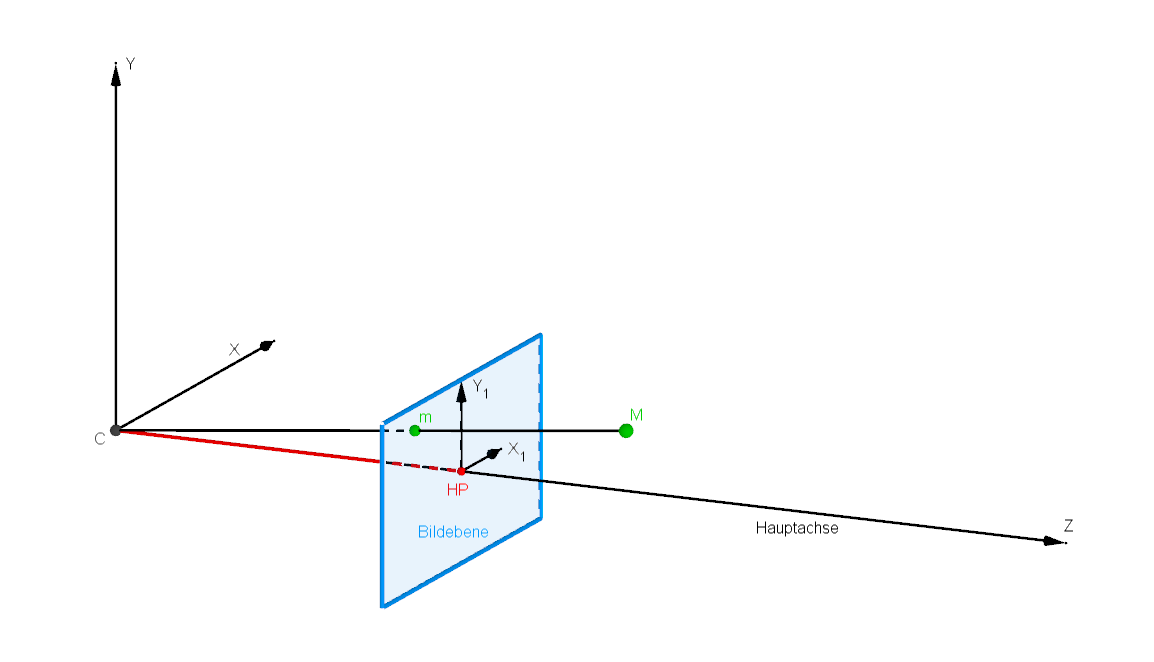
\includegraphics[width=.8\linewidth]{images/PinholeCameraModell3D.png}
%	\captionof{figure}{Schematik eines abbildenden Systems. Ein Punkt $M$ im  Weltkoordinatensystem $O$ wird durch eine Kamera $C$ aufgenommen. Diese Aufnahme wird durch eine Projektion, die als Verbindungslinie von $M$ zu $C$ zu sehen ist dargestellt ist und $M$ auf $m$ abbildet, beschrieben.}
%	\label{fig:PinholeCamera3D}
%\end{minipage}\\\\

Ein Punkt $M$ in einem dreidimensionalen Weltkoordinatensystem wird mit Hilfe einer Kamera, die in einem eigenen dreidimensionalen Kamerakoordinatensystem beschrieben wird, auf die Bildebene $I$ projiziert. Die Bildebene $I$ ist durch ein zweidimensionales Bildkoordinatensystem beschrieben. Der projizierte Punkt $m$ kann mit einem Sensor aufgenommen und abgespeichert werden.  \\ 

Im Folgenden wird zuerst ein Kameramodel eingeführt um die Projektion auf die Bildebene zu beschreiben. Daraufhin werden Koordinatentransformationen beschrieben um abschließend die Aufnahme eines Punktes mit einer willkürlichen Kameraorientierung zu berechnen. 


\section{Lochkameramodell zur Abbildung eines Punktes auf die Bildebene}

Mit Hilfe des Lochkameramodells wird die Abbildung eines Objektes auf eine Bildebene beschrieben. Das Modell beruht ausschließlich auf der geometrischen Optik und vernachlässigt physikalische Effekte, wie Beugung oder die Auswirkung der Linse\cite{Heipke}. Das Lochkameramodell besteht aus einem Projektionszentrum $C$. $C$ beschreibt gleichzeitig die Lage des Kamerazentrums und bildet den Ursprung des Kamerakoordinatensystems\cite{CamerModels.,HZ}. Die Blickrichtung der Kamera wird als Hauptachse bezeichnet. Die Bildebene steht senkrecht zur Hauptachse. Der Schnittpunkt der Hauptachse mit der Bildebene bildet den Hauptpunkt $HP$. Der Hauptpunkt ist der Ursprung des Bildebenenkoordinatensystems. Der Abstand vom Projektionszentrum zum Hauptpunkt wird als Brennweite $\zeta$ beschrieben\cite{HZ,CamerModels.}. Der Bildpunkt $m$ entsteht am Schnittpunk der Verbindungsgerade von $C$ und $M$ mit der Bildebene $I$. 

%\begin{minipage}{\linewidth}
%	\centering
%	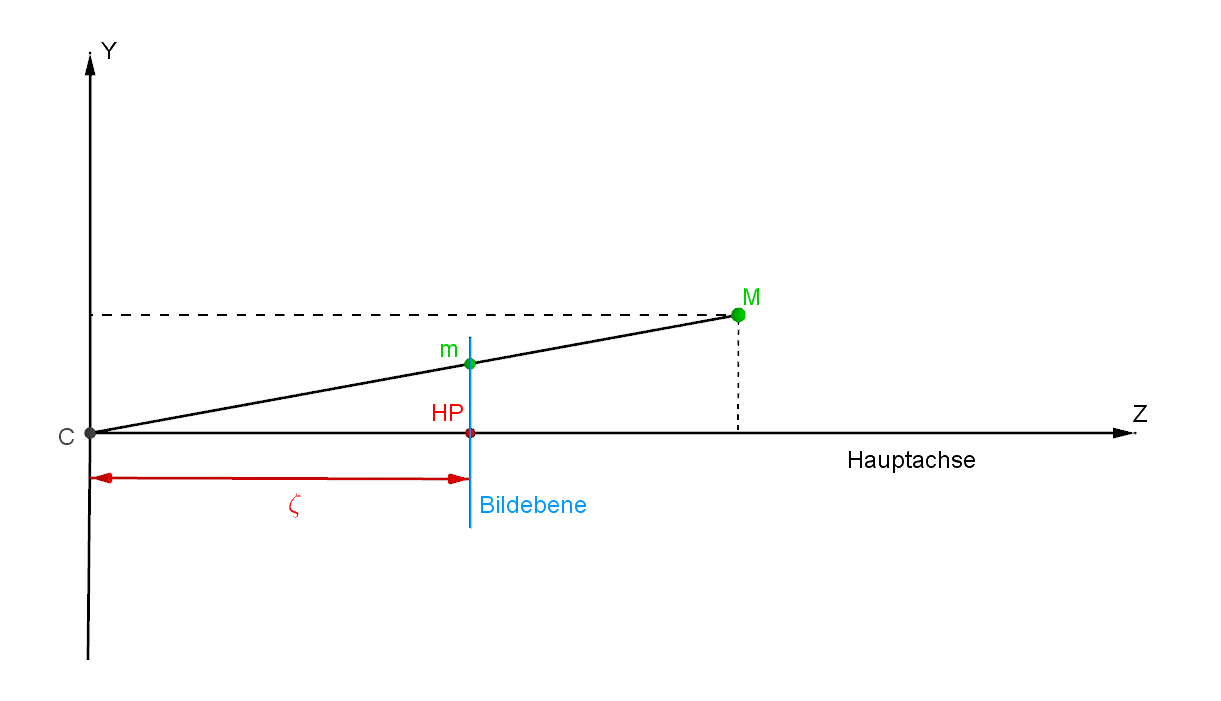
\includegraphics[width=.8\linewidth]{images/PinholeCameraModell2D.png}
%	\captionof{figure}{Die Abbildung zeigt einen Querschnitt des beschriebenen Lochkameramodells. Zu sehen ist das Projektionszentrum $C$ der Kamera. $C$ ist gleichzeitig das Kamerazentrum und bildet den Ursprung für das Kamerakoordinatensystem. $\zeta$ beschreibt den Abstand des Projektionszentrums zur Bildebene. Die Hauptachse beschreibt die Blickrichtung der Kamera. Der Punkt an dem die Hauptachse die Bildebene schneidet wird Hauptpunkt genannt und ist gleichzeitig der Ursprung für das Bildebenenkooridnatensystem. Der Bildpunkt $m$ entsteht am Schnittpunk der Verbindungsgerade von $C$ und $M$ mit der der Bildebene $I$}
%	\label{fig:PinholeCamera2D}
%\end{minipage}\\ \\


\begin{figure}[!htb]
	\centering
	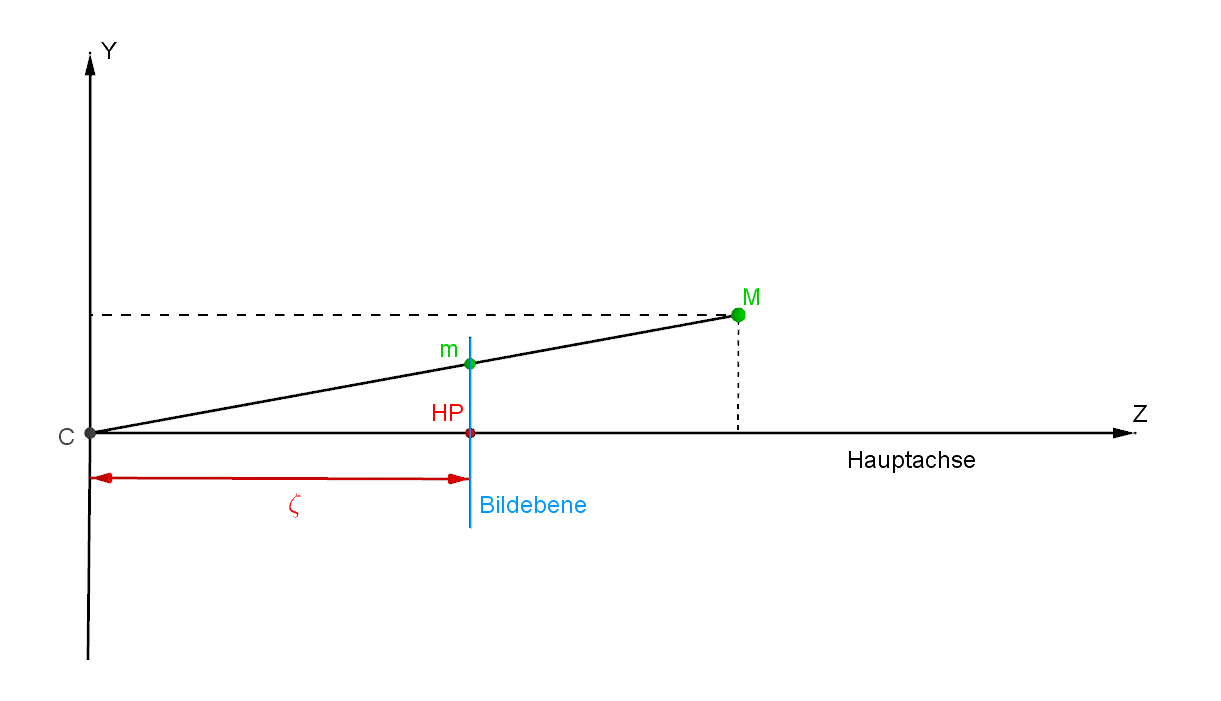
\includegraphics[width=.8\linewidth]{images/PinholeCameraModell2D.png}
	\caption[Lochkameramodell Querschnitt]{Die Abbildung zeigt einen Querschnitt des beschriebenen Lochkameramodells. Zu sehen ist das Projektionszentrum $C$ der Kamera. $C$ ist gleichzeitig das Kamerazentrum und bildet den Ursprung für das Kamerakoordinatensystem. $\zeta$ beschreibt den Abstand des Projektionszentrums zur Bildebene. Die Hauptachse beschreibt die Blickrichtung der Kamera. Der Punkt an dem die Hauptachse die Bildebene schneidet wird Hauptpunkt genannt und ist gleichzeitig der Ursprung für das Bildebenenkooridnatensystem. Der Bildpunkt $m$ entsteht am Schnittpunk der Verbindungsgerade von $C$ und $M$ mit der der Bildebene $I$}
	\label{fig:PinholeCamera2D}
\end{figure}

Die Projektion eines dreidimensionalen Punktes $M_\delta$ auf eine zweidimensionale Bildebene, wird durch eine $3 \times 3$ Kameramatrix $K_0$ beschrieben. 

\begin{gather}
	K_0\cdot M_\delta =
	\begin{bmatrix}
		\zeta&0&0\\
		0&\zeta&0\\
		0&0&1
	\end{bmatrix}
	\cdot
	\begin{bmatrix}
		X\\Y\\Z
	\end{bmatrix}
	=
	\begin{pmatrix}
		\zeta X\\ \zeta Y\\ Z
	\end{pmatrix}
	\mapsto
	\begin{pmatrix}
		\zeta \frac{X}{Z}\\ \zeta \frac{Y}{Z}
	\end{pmatrix}
	\label{eq:2.1}
\end{gather}\\

Die Koordinaten auf der zweidimensionalen Bildebene werden häufig als homomogene Koordinaten angegeben. Dazu werden die Koordinaten mit $Z$ normiert und somit auf die Ebene $(x,y,1)^T$ projiziert wird. Zur Vereinfachung wird zuletzt nur die $x,\,y$ Koordinaten des entstandenen Bildes angegeben. Gleichung \ref{eq:2.1} beschreibt somit die Abbildung eines Punktes auf die Bildebene.
%Die Kameramatrix beinhaltet alle Informationen über die intrinsischen Kameraparameter einer Kamera. $\zeta$ ist ein intrinsischer Kameraparameter. Mit $\zeta$ kann ein dreidimensionaler Punkt  $M=[X\,Y\,Z]$ in Kamerakoordinaten in einen Punkt $m$ in Bildebenenkoordinaten projiziert werden.

\section{Koordinatentransformation}

Um einen Punkt von einem übergeordneten Weltkoordinatensystem in ein bestimmtes, zum Weltkoordinatensystem rotiertes, Kamerakoordinatensystem zu überführen ist eine Transformation notwendig. Im Folgenden wird der mathematische Weg einer Transformation eines Weltkoordinatensystems $(O,\delta)$ mit $\delta = (\hat{d_1},\hat{d_2},\hat{d_3},O)$ in ein Kamerakoordinatensystem $(C,\beta)$ mit $\beta = (\hat{b_1},\hat{b_2},\hat{b_3},C)$ beschrieben.



\begin{figure}[!htb]
	\centering
	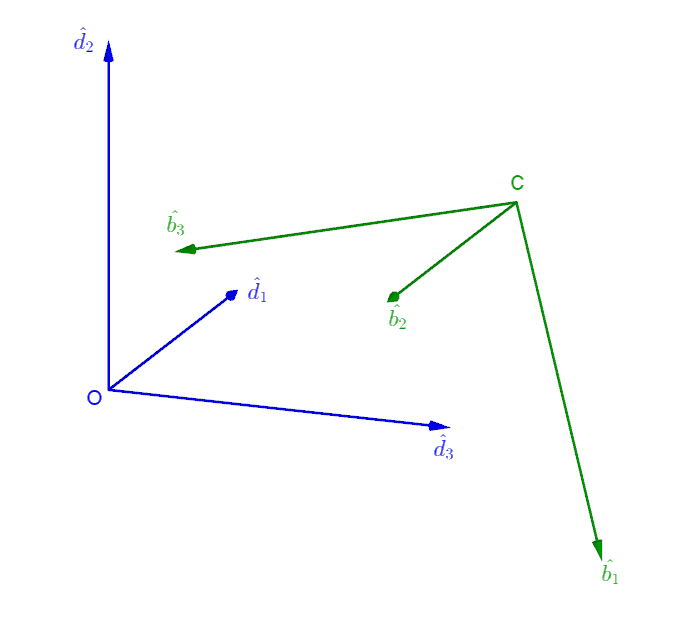
\includegraphics[width=0.7\linewidth]{images/WeltKordSys.png}
	\caption[Koordinatentransformation]{Ein Weltkoordinatensystem $(O,\delta)$ mit $\delta = (\hat{d_1},\hat{d_2},\hat{d_3},O)$ wird zu einem dazu verschobenen und rotiertem Kamerakoordinatensystem  $(C,\beta)$ mit $\beta = (\hat{b_1},\hat{b_2},\hat{b_3},C)$ transformiert.}
	\label{fig:Koordinatensysteme1}
\end{figure}

%\begin{minipage}{\linewidth}
%	\centering
%	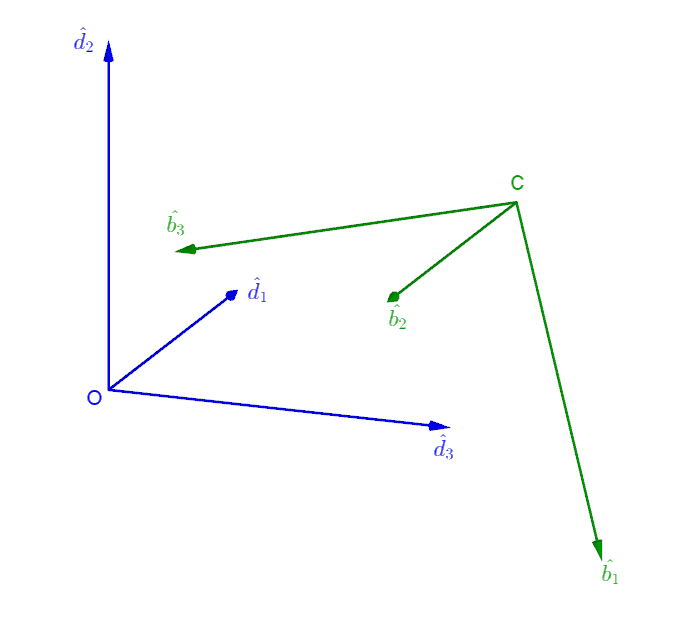
\includegraphics[width=0.7\linewidth]{images/WeltKordSys.png}
%	\captionof{figure}{Ein Weltkoordinatensystem $(O,\delta)$ mit $\delta = (\hat{d_1},\hat{d_2},\hat{d_3},O)$ wird zu einem dazu verschobenen und rotiertem Kamerakoordinatensystem  $(C,\beta)$ mit $\beta = (\hat{b_1},\hat{b_2},\hat{b_3},C)$ transformiert}
%	\label{fig:Koordinatensysteme1}
%\end{minipage}\\ \\

Zunächst wird eine Koordinatisierung von Punkten im Weltkoordinatensystem vorgenommen. Ein Punkt $P_\delta$ bezüglich des Weltkoordinatensystems wird wie folgt beschrieben


\begin{gather}
	P_\delta = O + p_{\delta x}\,\hat{d_1} + p_{\delta y}\,\hat{d_2} + p_{\delta z}\,\hat{d_3}\label{eq:eq2.2}\\
	\leadsto P_\delta = (p_{\delta x},p_{2\delta y},p_{\delta z})^T = \begin{pmatrix} p_{\delta x} \\ p_{\delta y} \\ p_{\delta z} \end{pmatrix}.
\end{gather}

Zwischen den beiden Koordinatensystemen	$(O,\delta)$  und $(C,\beta)$ gelten die folgenden Beziehungen

\begin{gather}
	C_\beta = O_\delta + C_{\beta,1}\,\hat{d_1} +C_{\beta,2}\,\hat{d_2} + C_{\beta,3}\,\hat{d_3}\\
	\hat{b_1} = b_{11}\,\hat{d_1} +  b_{12}\,\hat{d_2} +  b_{13}\,\hat{d_3}\\
	\hat{b_2} = b_{21}\,\hat{d_1} +  b_{22}\,\hat{d_2} +  b_{23}\,\hat{d_3}\\
	\hat{b_3} = b_{31}\,\hat{d_1} +  b_{32}\,\hat{d_2} +  b_{33}\,\hat{d_3}.
\end{gather}

Diese Beziehungsgleichungen werden in Gleichung \ref{eq:eq2.2} eingesetzt.

\begin{gather}
	\begin{split}
		P_\delta = O + (C_{\beta,1} + p_{\beta x}\,b_{11} +  p_{\beta y}\,b_{21} + p_{\beta z}\,b_{31}) \cdot \hat{d_1}\\
		+(C_{\beta,2} + p_{\beta x}\,b_{21} +  p_{\beta y}\,b_{22} + p_{\beta z}\,b_{32} )\cdot \hat{d_2}\\
		+ (C_{\beta,3} + p_{\beta x}\,b_{31} +  p_{\beta y}\,b_{23} + p_{\beta z}\,b_{33} )\cdot \hat{d_3}.\label{eq:2.8}
	\end{split}
\end{gather}

Aus Gleichung \ref{eq:2.8} wird ein Gleichungssystem in der Form von Gleichung \ref{eq:2.9} aufgestellt und gelöst.

\begin{gather}
	\begin{split}
		p_{\delta x} = C_{\beta,1} + (C_{\beta,1} + p_{\beta x}\,b_{11} +  p_{\beta y}\,b_{21} + p_{\beta z}\,b_{31} \\
		\leadsto \: p_{\delta x} - C_{\beta,1} =  (C_{\beta,1} + p_{\beta x}\,b_{11} +  p_{\beta y}\,b_{21} + p_{\beta z}\,b_{31}).\label{eq:2.9}
	\end{split}
\end{gather}

Das Gleichungssystem lässt sich in Matrixform darstellen als 

\begin{gather}
	\begin{bmatrix}b_{11} & b_{21} & b_{31}\\
		b_{12} & b_{22} & b_{32}\\
		b_{13} & b_{23} & b_{33}
	\end{bmatrix} 
	\begin{pmatrix}
		p_{\beta x}\\p_{\beta y}\\ p_{\beta z}
	\end{pmatrix} = 
	\begin{pmatrix}
		p_{\delta x} - C_{\beta,1}\\
		p_{\delta y} - C_{\beta,2}\\
		p_{\delta z} - C_{\beta,3}
	\end{pmatrix}.
\end{gather}\\

Wenn $P_\beta$ gegeben ist, erhält man auf diese Weise direkt $P_\delta$. Die inverse Matrix $\ensuremath{D_\beta^{-1}}$ kann verwendet werden um  $P_\beta$ aus $P_\delta$ zu berechnen.

\begin{gather}
	D_\beta^{-1} = 
	\begin{bmatrix}b_{11} & b_{12} & b_{13}\\
		b_{21} & b_{22} & b_{23}\\
		b_{31} & b_{32} & b_{33}
	\end{bmatrix}\\
	\begin{split}
		\leadsto \: \begin{pmatrix}
			p_{\beta x}\\p_{\beta y}\\ p_{\beta z}
		\end{pmatrix}
		= D_\beta^{-1} 
		\begin{pmatrix}
			p_{\delta x} - C_{\beta,1}\\
			p_{\delta y} - C_{\beta,2}\\
			p_{\delta z} - C_{\beta,3}
		\end{pmatrix}.\label{eq:2.12}
	\end{split} 
\end{gather}

Handelt es sich um ein kartesisches Koordinatensystem, so gilt $\ensuremath{D_\beta^{-1}}=D_\beta^{T}$ und die transponierte Matrix kann für die Koordinatentransformation benutzt werden. Für zwei normierte, kartesische Koordinatensysteme ist $D$ und $D^T$ eine Rotationsmatrix $R$, weshalb im Folgenden, analog zur Literatur \cite{HZ,Elements,Ferid}, $D^T=R$ angenommen wird.  Um Gleichung \ref{eq:2.12} in einer kompakten Schreibweise zu formulieren, wird $\overrightarrow{p_{\beta}}=(p_{\beta x},p_{\beta y},p_{\beta z})^T$ zu einem vierdimensionalen Vektor mit 1 zu $\overrightarrow{p_{\beta4}}=(p_{\beta x},p_{\beta y},p_{\beta z},1)^T=(\overrightarrow{p_{\beta}},1)^T$ erweitert. Damit lässt sich Gleichung \ref{eq:2.12} als eine Matrixmultiplikation ausdrücken

\begin{gather}
	\begin{pmatrix}
		p_{\beta x}\\p_{\beta y}\\ p_{\beta z}
	\end{pmatrix}
	= D_\beta^T	
	\begin{bmatrix}1 & 0 & 0 & - C_{\beta,1}\\
		0 & 1 & 0& - C_{\beta,2}\\
		0 & 0 & 1 & - C_{\beta,3}
	\end{bmatrix} 
	\begin{pmatrix}
		p_{\delta x}\\p_{\delta y}\\ p_{\delta z}\\1
	\end{pmatrix}
	= R	[I -C] 	 \begin{pmatrix}
		p_{\delta x}\\p_{\delta y}\\ p_{\delta z}\\1
	\end{pmatrix}
	= T	\begin{pmatrix}
		\vec{p_\delta}\\1
	\end{pmatrix}.	 \label{eq:trafo}
\end{gather}

Die Transformationsmatrix $T$ setzt sich aus der Rotationsmatrix $R$ und der Translationsmatrix  $[I |-C]$ zusammen und wirkt auf den neu definierten vierdimensionalen Vektor. Wichtig dabei ist, dass $[I| -C]$ eine symbolische Schreibweise für eine $3 \times 4$ Matrix ist.   

%Einmal wird wie bereits angefangen mit Spaltenvektoren gearbeitet, das selbe Verfahren wird dann noch einmal mit Zeilenvektoren dargestellt.  Beide Ansätze funktionieren nach dem selben Prinzip. Der Unterschied ist die Darstellung der Matrizen.

%Beim arbeiten mit Programmen wie Beispielsweise \textit{Matlab} ist es wichtig zu wissen, ob mit Spalten oder Zeilenvektoreden gearbeitet wird. \textit{MatLab} arbeitet mit Spaltenvektoren, während entwickelten Algorithmus dieser Arbeit mit Zeilenvektoren gearbeitet wurde. Zunächst wird also weiter mit Spaltenvektoren verfahren. 
%Wir nehmen an, dass der Punkt  $\beta = (\hat{b_1},\hat{b_2},\hat{b_3},C)$ im Kamerakoordinatensystem und der Punkt $\delta = (\hat{d_1},\hat{d_2},\hat{d_3},O)$ im Weltkoordinatensystem identisch sind. Die Koordinatensystem sind zueinander rotiert und der Ursprung des Kamerakoordinatensystems ist bezüglich des Ursprungs des Weltkoordiantensystems verschoben. Der Translationsvektor entspricht den Koordinaten des Ursprungs des Kamerakoordinatensystem $\vec{V} = C_\beta = (C_{\beta,1}, C_{\beta,2}, C_{\beta,3})^T$. Die Transformation lässt sich in diesem vierdimensionalen Raum ausdrücke als  
%welche aus der Rotation $D$ und dem Translationsvektor $\vec{V}$ ensteht, wird im weiteren Verlauf mit $R$ bezeichnet. $R$ fasst die extrinsischen Kameraparameter in einer Matrix zusammen.

%	\begin{gather}
%	\begin{pmatrix}
%		\hat{b_1}\\
%		\hat{b_2}\\
%		\hat{b_3}\\
%		C_\beta
%	\end{pmatrix} = 
%	\begin{bmatrix}
%		b_{11} & b_{21} & b_{31} & 0\\
%		b_{12} & b_{22} & b_{32} & 0\\
%		b_{13} & b_{23} & b_{33} & 0\\
%		C_{\beta,1} & C_{\beta,2} & C_{\beta,3} & 1 
%	\end{bmatrix}
%	\begin{pmatrix}
%		\hat{d_1}\\
%		\hat{d_2}\\
%		\hat{d_3}\\
%		O_\delta
%	\end{pmatrix}
%	= R\delta\\.
%\end{gather}
%Die Transformationsmatrix $R$ setzte sich aus den Komponenten der Rotationsmatrix aus Gleichung \ref{2.10} und dem Translationsvektor $\vec{V}$ zusammen. Diese Parameter beschreiben die Kameraposition und Kameraorientierung, welche als extrinsische Kameraparameter bekannt sind.    

%Für eine Rücktransformation von Kamera in Weltkoordinaten muss die Inverse von R gebildet werden. %Diese Inverse lässt sich in karthesischen Koordinaten durch die transponierten Rotationsmatrix D %und der Inversen des Translationsvektor $\vec{V}$ wie folgt ausdrücken.

%\begin{gather}
%	\leadsto \: \begin{pmatrix}
%		\hat{d_1}\\
%		\hat{d_2}\\
%		\hat{d_3}\\
%		O_\delta
%	\end{pmatrix} = 
%	\begin{bmatrix}
%		b_{11} & b_{21} & b_{31} & 0\\
%		b_{12} & b_{22} & b_{32} & 0\\
%		b_{13} & b_{23} & b_{33} & 0\\
%		&-(	C_{\beta,1}, C_{\beta,2}, C_{\beta,3})C^{-1}& & 1
%	\end{bmatrix}
%	\begin{pmatrix}
%		\hat{b_1}\\
%		\hat{b_2}\\
%		\hat{b_3}\\
%		C_\beta
%	\end{pmatrix}
%\end{gather}

%Das selbe Verfahren mit Zeilenvektoren führt zu den Gleichungen 2.24 und 2.25.

%\begin{gather}
%	(\hat{b_1}, \hat{b_2}, \hat{b_3}, C_\beta) = (\hat{d_1},\hat{d_2}, \hat{d_3}, O) \cdot
%	\begin{bmatrix} 
%		b_{11} & b_{21} & b_{31} & C_{\beta,1}\\
%		b_{12} & b_{22} & b_{23} & C_{\beta,2}\\
%		b_{13} & b_{32} & b_{33} & C_{\beta,2}\\
%		0           &       0       &   0         & 1   
%	\end{bmatrix}
%\end{gather}	

%Daraus folgt, dass für den Fall der Rücktransformation gilt:

%\begin{gather}
%	\leadsto \: \begin{pmatrix}
%		\hat{d_1},\hat{d_2},\hat{d_3},O
%	\end{pmatrix} = 
%		\begin{pmatrix}
%	\hat{b_1},\hat{b_2},\hat{b_3},C_\beta
%	\end{pmatrix}
%	\begin{bmatrix}
%		b_{11} & b_{12} & b_{13} & \\
%		b_{21} & b_{22} & b_{23} &  -\begin{pmatrix}
%			C_{\beta,1}\\
%			C_{\beta,2}\\
%			C_{\beta,3}
%		\end{pmatrix}C^{-1}\\
%		b_{31} & b_{32} & b_{33} & \\
%		0&0&0 & 1
%	\end{bmatrix}
%\end{gather}	

\pagebreak


\section{Aufnahme mit einer willkürlichen Kameraorientierung}

Ein beliebiger Punkt im Weltkoordinatensystem kann mit der eingeführten Operation auf die Bildebene und schließlich auch auf den Sensor projiziert werden. Es werden insgesamt vier verschiedene Koordinatensysteme definiert.
Das Weltkoordinatensystem $(O,\delta)$ mit $\delta =(\hat{d_1}, \hat{d_2},\hat{d_3})$, das Kamerakoordinatensystem $(C,\beta)$ mit $\beta = (\hat{b_1},\hat{b_2},\hat{b_3})$, das Bildebenenkoordinatensystem $(I,\tau)$ mit $\tau = (\hat{t_1},\hat{t_2})$ und als letztes das Sensorkoordinatensystem mit $(S,\sigma)$ mit $\sigma = (\hat{u},\hat{v})$. Abbildung \ref{fig:KoordinatensystemeUeberblick} zeigt die Koordinatensysteme schematisch im Überblick. 


\begin{figure}[!htb]
	\centering
	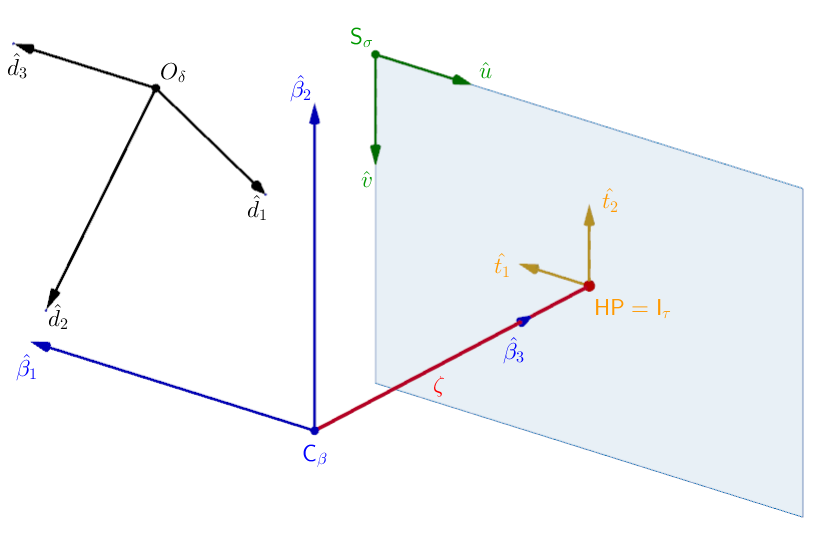
\includegraphics[width=0.8\linewidth]{images/UebersichtKoordinatensysteme_beschriftet.png}
	\caption[Koordinatensysteme im Überblick]{Das Schaubild zeigt die einzelnen Koordinatensysteme in einem Lochkameramodell. Das Weltkoordinatensystem $(O,\delta)$ mit $\delta = (\hat{d_1},\hat{d_2},\hat{d_3})$, das Kamerakoordinatensystem $(C,\beta)$ mit $\beta = (\hat{b_1},\hat{b_2},\hat{b_3})$, das Bildebenenkoordinatensystem $(I,\tau)$ mit $\tau = (\hat{t_1},\hat{t_2})$ und das Sensorkoordinatensystem $(S,\sigma)$ mit $\sigma = (\hat{u},\hat{v})$. }
	\label{fig:KoordinatensystemeUeberblick}
\end{figure}

%\begin{minipage}{\linewidth}
%	\centering
%	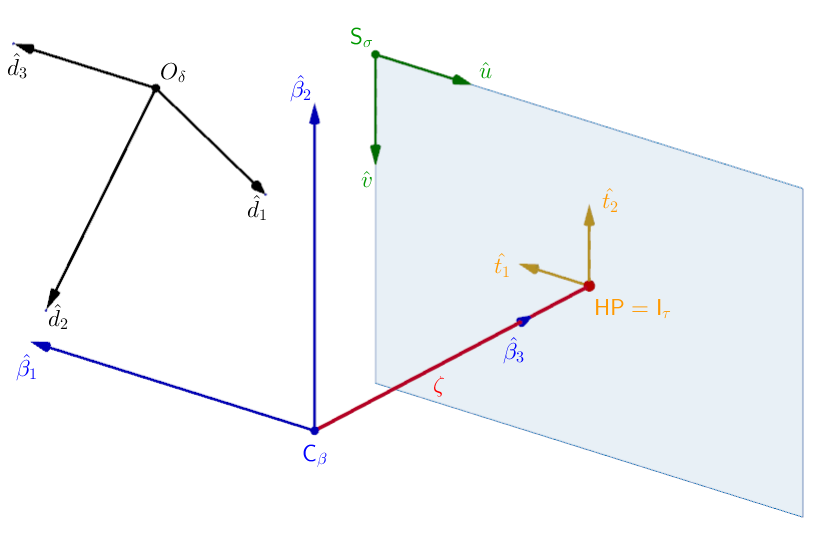
\includegraphics[width=0.8\linewidth]{images/UebersichtKoordinatensysteme_beschriftet.png}
%	\captionof{figure}{Das Schaubild zeigt die einzelnen Koordinatensysteme in einem Lochkameramodell. Das Weltkoordinatensystem $(O,\delta)$ mit $\delta = (\hat{d_1},\hat{d_2},\hat{d_3})$, das Kamerakoordinatensystem $(C,\beta)$ mit $\beta = (\hat{b_1},\hat{b_2},\hat{b_3})$, das Bildebenenkoordinatensystem $(I,\tau)$ mit $\tau = (\hat{t_1},\hat{t_2})$ und das Sensorkoordinatensystem $(S,\sigma)$ mit $\sigma = (\hat{u},\hat{v})$. }
%	\label{fig:KoordinatensystemeUeberblick}
%\end{minipage}\\ \\ 

Für die Projektion eines Punktes $M_\delta=({M_{\delta x}}\,{M_{\delta y}}\,{M_{\delta z}})^T$ bezüglich des Weltkoordinatensystems in einen Punkt $m_\tau=({m_{\tau x}}\,{m_{\tau y}}\,{m_{\tau z}})^T$ bezüglich des Bildebenenkoordinatensystems kann eine Projektionsmatrix $P$ definiert werden.\\

Zuerst muss der Punkt im Weltkoordinatensystem in das Kamerakoordinatensystem transformiert werden. Für die Transformation der Weltkoordinaten in Kamerakoordinaten gilt die Gleichung \ref{eq:trafo}
\begin{equation}
\overrightarrow{M_\beta}=T
\begin{bmatrix}
\overrightarrow{M_\delta}\\
1\\
\end{bmatrix}=R \begin{bmatrix}1 & 0 & 0 & - C_{\beta x}\\
0 & 1 & 0& - C_{\beta y}\\
0 & 0 & 1 & - C_{\beta z}
\end{bmatrix} 
\begin{pmatrix}
M_{\delta x}\\M_{\delta y}\\ M_{\delta z}\\1
\end{pmatrix}
=R	[I -C] \begin{bmatrix}
\vec{M_\delta}\\
1\\
\end{bmatrix}. \label{mbeta}
% ({M_{Cx}}\,{M_{Cy}}\, {M_{Cz}}\, C_{\beta})=({M_{Ox}}\,{M_{Oy}}\,{M_{Oz}}\,O_{\delta}) \cdot R
\end{equation}

Nach der Transformation eines Punkts $\overrightarrow{M_\delta}$ zu $\overrightarrow{M_\beta}$ in das Kamerakoordinatensystem erfolgt die Kameraprojektion von $M_\beta$ auf $m_\beta$ wie in Gleichung \ref{eq:2.1} beschrieben. %Die Kameramatrix lässt den Ursprung eines Koordinatensystems unverändert und die Kameramatrix $K_0$ lässt sich erweitern:
\begin{equation}
\begin{bmatrix}
m_{\beta x}\\m_{\beta y}\\m_{\beta z}
\end{bmatrix} = \begin{bmatrix}
\zeta&0&0\\
0&\zeta&0\\
0&0&1
\end{bmatrix}
\begin{bmatrix}
M_{\beta x}\\M_{\beta y}\\M_{\beta z}
\end{bmatrix}
=K_0\overrightarrow{M_{\beta}}\label{mbeta1}.
\end{equation}
\pagebreak

Die Projektion eines Punktes $\overrightarrow{M_\delta}$ auf den Bildpunkt $\overrightarrow{m_{\beta}}$ kann durch Gleichung \ref{mbeta} und \ref{mbeta1} zusammengefasst werden

\begin{equation}
\overrightarrow{m_\beta}
=K_0 R	[I -C] \begin{bmatrix}
\overrightarrow{M_\delta}\\
1\\
\end{bmatrix} .
% ({M_{Cx}}\,{M_{Cy}}\, {M_{Cz}}\, C_{\beta})=({M_{Ox}}\,{M_{Oy}}\,{M_{Oz}}\,O_{\delta}) \cdot R
\end{equation}


Um den Bildpunkt $\overrightarrow{m_{\beta}}$ bezüglich eines zweidimensionalen Bildebenenkoordinatensystemes anzugeben, wird die Bildebene mit der Tiefkomponente $m_{\beta z}$ normiert, sodass $m_{\beta z}$ auf den zweidimensionalen Raum der Bildebene abgebildet wird. Diese Projektion wird durch folgende Gleichung beschrieben

\begin{equation}
\overrightarrow{m_\tau} =
\begin{bmatrix}
m_{\beta x}/m_{\beta z}\\m_{\beta y}/m_{\beta z}\\1
\end{bmatrix}.
\end{equation}


Zuletzt folgt die Transformation der Bildebenenkoordinaten auf den Sensorchip. Der Sensorchip besteht aus einer Ansammlung von Sensorelementen. Diese Sensorelemente können verschiedene Formen annehmen. Die meisten Sensorchips bestehen aus rechtwinkligen, rechteckigen Sensorelementen. Aus diesem Grund wird ein rechtwinkliges Sensorelement mit einer Größe $lx$ $ly$ angenommen. Diese Sensorelementgröße $lx$ $ly$ definiert auch die Pixelgröße und bildet die Längenskalierung des Sensorkoordinatensystems. Neben der unterschiedlichen Skalierung wird der Ursprung des Sensorkoordinatensystems in der Regel an einer Ecke des Sensorchips definiert, sodass die Transformation von Bildebenenkoordinaten in Sensorkoordinaten auch eine Translation $(V_{\sigma x},V_{\sigma y})$ aufweist\cite{HZ,Photonik}. Für einen Punkt $m_\sigma = ({u},{v},1)$ auf dem Sensorkoordinatensystem lassen sich die folgenden Bedingungen herleiten 

\begin{gather}	
	{u}=m_{\tau x} \, k_x - V_{\sigma x}\\
	{v}=m_{\tau y} \, k_y - V_{\sigma y}\\
	1=1\,.
\end{gather}


$k_x=1/lx$ und $k_y=1/ly$ ist die Pixeldichte in $\frac{pixel}{mm}$. Es wird angemerkt, dass in der Bildebene und der Sensorebene die Punkte ausschließlich im zweidimensionalen Raum definiert sind. Aus den normierten Bildkoordinaten lässt sich somit folgende Sensormatrix bilden

\begin{gather}
	\overrightarrow{m_\sigma}=\begin{bmatrix}u \\v\\1 \end{bmatrix}=
	\begin{bmatrix}
		k_x&0&V_{\sigma x}\\
		0&k_y&V_{\sigma y}\\
		0&0&1&\\
	\end{bmatrix}
	\begin{bmatrix}m_{\tau x}\\ m_{\tau y}\\ 1\end{bmatrix}= R_\sigma \vec{m_\tau}\,.
\end{gather}

Mit Hilfe der Transformationsmatrix $R_\sigma$ kann ein Punkt von der Bildebene auf das Sensorelement projiziert werden.\\

Der hier skizzierte Lösungsweg beschreibt die Bildaufnahme eines Punktes im Lochkameramodel. Die hier eingeführte Projektionsmatrix $P=K_0R[I -C]$ gilt für die Abbildung eines Punktes auf den Bildpunkt. Der Bildpunkt wird normiert und in das Sensorkoordinatensystem umgerechnet. In der Literatur wird häufig die Transformation in das Sensorkoordinatensystem bereits in der Kameramatrix zusammengefasst. Damit bildet sich die erweiterte Kameramatrix $K$

\begin{equation}
K=	R_\sigma K_0=  \begin{bmatrix}
k_x \zeta & 0 & V_{\sigma x}\\
0 & k_y \zeta & V_{\sigma y}\\
0 & 0   & 1 &\\
\end{bmatrix}.
\end{equation}

Mit dieser Kameramatrix wird eine neue Projektionsmatrix mit $P=KR[I -C]$ gebildet, die einen Objektpunkt auf einen Bildpunkt im Sensorkoordinatensystem abbildet. Durch die Normierung dieses Punktes kann auf den direkten Sensorpunkt geschlossen werden.  Ein weiterer Vorteil der erweiterten Kameramatrix $K$ ist, dass sie die Pixeldichte $k_x,k_y$ und die Brennweite $\zeta$ beinhaltet. Diese Parameter werden im Folgenden als intrinsische Kameraparameter bezeichnet. Die Koordinatentransformationsmatrix $R$ wird im Gegensatz aus den sogenannten extrinsischen Kameraparameter, der Kameraposition und Orientierung, definiert. Sind sowohl die intrinsischen wie auch extrinsischen Kameraparameter vorbestimmt kann $P$ bestimmt und mit dem hier beschriebenen Lösungsweg das Bild konstruiert werden. % ein Punkt auf die Sensorebene der entsprechenden Kamera projeziert werden. 


%Die Prokjektionsmatrix $P=RK_0R_\sigma$ setzt sich aus einer Koordinatentransformationsmatirx $R$, der Kameramatrix $K_0$ und einer weiteren Transformation zusammen. Häufig werdend die letzten beiden Matrizen zu einer erweiterten Kameramatrix $K=K_0R_\sigma$ zusammengefasst. Die erweiterte Kameramatrix beinhaltet die Pixeldichte $k_x,k_y$ und die Brennweite $\zeta$. Diese Parameter werden im folgenden als intrinsische Kameraparameter bezeichnet. Die Koordinatentransformationsmatrix $R$ wird im gegensatz aus den sogenannten extrinsischen Kameraparameter, der Kameraposition und Orientierung, definiert. Sind sowohl die intrinsischen wie auch extrinsischen Kameraparameter vorbestimmt kann somit $P$ bestimmt werden und ein Punkt auf die Sensorebene der entsprechenden Kamera projeziert werden. 

%Die Kamermatrix K_0 wird mit der Koordinatentransformation in das Sensorkoordinatensystem zu einer Erweiterten Kameramatrix K zusammengefasst. Die Einträge in dieser ERweiterten Kameramatrix ....

